% PGFPlots Showcase (based on TODO/graph-plot.md)
\documentclass[11pt]{article}
\usepackage[a4paper,margin=1in]{geometry}
\usepackage{amsmath}
\usepackage{pgfplots}
\pgfplotsset{compat=1.18}

\title{PGFPlots Showcase}
\author{LaTeX Research Toolkit}
\date{2D/3D plots, domains, ticks, and data-driven charts}

\begin{document}
\maketitle

\section{Basic 2D Function}
\begin{tikzpicture}
  \begin{axis}[axis lines=middle, xmin=-2, xmax=2, ymin=-2, ymax=2,
               xlabel={$x$}, ylabel={$y$}, title={Cubic}]
    \addplot[color=red, thick, samples=100, domain=-2:2] {x^3};
  \end{axis}
\end{tikzpicture}

\section{Custom Ticks and Grid}
\begin{tikzpicture}
  \begin{axis}[axis lines=middle, xmin=0, xmax=3.2, ymin=-1.5, ymax=1.5,
               xtick={0, 1.57, 3.14},
               xticklabels={0, $\frac{\pi}{2}$, $\pi$},
               ytick={-1,0,1}, xmajorgrids=true,
               title={Sine with Custom Ticks}]
    \addplot[blue, thick, samples=150, domain=0:3.14] {sin(deg(x))};
  \end{axis}
\end{tikzpicture}

\section{Stacked Bar Chart}
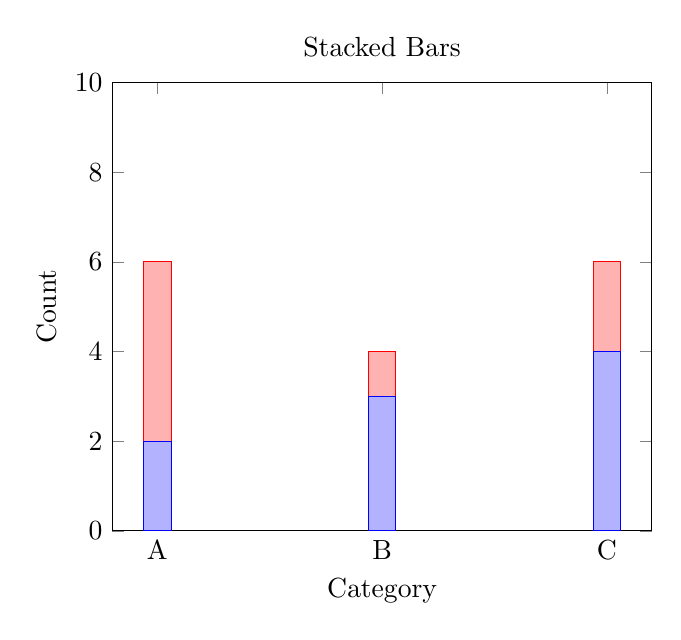
\begin{tikzpicture}
  \begin{axis}[ybar stacked, ymin=0, ymax=10,
               xlabel={Category}, ylabel={Count},
               symbolic x coords={A,B,C}, xtick=data,
               title={Stacked Bars}]
    \addplot coordinates {(A,2) (B,3) (C,4)};
    \addplot coordinates {(A,4) (B,1) (C,2)};
  \end{axis}
\end{tikzpicture}

\section{3D Surface}
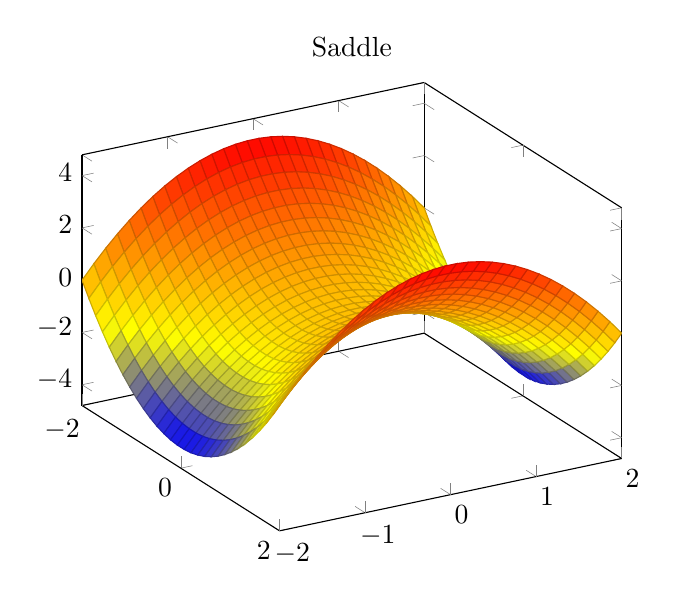
\begin{tikzpicture}
  \begin{axis}[view={60}{30}, title={Saddle}]
    \addplot3[surf, samples=30, domain=-2:2, domain y=-2:2] {x^2 - y^2};
  \end{axis}
\end{tikzpicture}

\section{Data-Driven Plot (CSV)}
% Uses examples/basic/data.csv with headers: Name,Score,Passed
\begin{tikzpicture}
  \begin{axis}[
    ybar, ymin=0, ymax=100,
    xlabel={Name}, ylabel={Score},
    symbolic x coords={Alice,Bob,Carol,Dave}, xtick=data,
    title={Scores from CSV}
  ]
    \addplot+[
      only marks, mark=*, mark size=2pt,
    ] table[x=Name,y=Score,col sep=comma]{../basic/data.csv};
  \end{axis}
\end{tikzpicture}

\end{document}
